\documentclass[a4paper]{article}
\usepackage[utf8]{inputenc}
\usepackage[T1]{fontenc}
\usepackage[spanish]{babel}
\usepackage{a4wide}
\usepackage{amsmath}
\usepackage{amssymb,amsfonts,textcomp}
\usepackage{color}
\usepackage{array}
\usepackage{supertabular}
\usepackage{hhline}
\usepackage{hyperref}
\usepackage{fancyhdr}
\usepackage[table]{xcolor}
%\hypersetup{pdftex, colorlinks=true, linkcolor=blue, citecolor=blue, filecolor=blue, urlcolor=blue, pdftitle=, pdfauthor=, pdfsubject=, pdfkeywords=}
\usepackage[pdftex]{graphicx}
% footnotes configuration
\makeatletter
\renewcommand\thefootnote{\arabic{footnote}}
\makeatother
% Text styles
\newcommand\textstyleStrongEmphasis[1]{\textbf{#1}}
% Outline numbering
\setcounter{secnumdepth}{0}
\makeatletter
\newcommand\arraybslash{\let\\\@arraycr}
\makeatother
% List styles
\newcommand\liststyleWWNumxxix{%
\renewcommand\labelitemi{{}-}
\renewcommand\labelitemii{o}
\renewcommand\labelitemiii{[F0A7?]}
\renewcommand\labelitemiv{[F0B7?]}
}
\newcommand\liststyleLi{%
\renewcommand\labelitemi{{\textbullet}}
\renewcommand\labelitemii{${\circ}$}%
\renewcommand\labelitemiii{${\blacksquare}$}
\renewcommand\labelitemiv{{\textbullet}}
}
\newcommand\liststyleLii{%
\renewcommand\labelitemi{{\textbullet}}
\renewcommand\labelitemii{${\circ}$}
\renewcommand\labelitemiii{${\blacksquare}$}
\renewcommand\labelitemiv{{\textbullet}}
}
\newcommand\liststyleLiii{%
\renewcommand\labelitemi{{\textbullet}}
\renewcommand\labelitemii{${\circ}$}
\renewcommand\labelitemiii{${\blacksquare}$}
\renewcommand\labelitemiv{{\textbullet}}
}
\newcommand\liststyleLiv{%
\renewcommand\labelitemi{{\textbullet}}
\renewcommand\labelitemii{${\circ}$}
\renewcommand\labelitemiii{${\blacksquare}$}
\renewcommand\labelitemiv{{\textbullet}}
}
\newcommand\liststyleLv{%
\renewcommand\labelitemi{{\textbullet}}
\renewcommand\labelitemii{${\circ}$}
\renewcommand\labelitemiii{${\blacksquare}$}
\renewcommand\labelitemiv{{\textbullet}}
}
\newcommand\liststyleLvi{%
\renewcommand\labelitemi{{\textbullet}}
\renewcommand\labelitemii{${\circ}$}
\renewcommand\labelitemiii{${\blacksquare}$}
\renewcommand\labelitemiv{{\textbullet}}
}
\newcommand\liststyleLvii{%
\renewcommand\labelitemi{{\textbullet}}
\renewcommand\labelitemii{{\textbullet}}
\renewcommand\labelitemiii{{\textbullet}}
\renewcommand\labelitemiv{{\textbullet}}
}
\newcommand\liststyleLviii{%
\renewcommand\labelitemi{{\textbullet}}
\renewcommand\labelitemii{{\textbullet}}
\renewcommand\labelitemiii{{\textbullet}}
\renewcommand\labelitemiv{{\textbullet}}
}
\newcommand\liststyleLix{%
\renewcommand\labelitemi{{\textbullet}}
\renewcommand\labelitemii{{\textbullet}}
\renewcommand\labelitemiii{{\textbullet}}
\renewcommand\labelitemiv{{\textbullet}}
}
\newcommand\liststyleLx{%
\renewcommand\labelitemi{{\textbullet}}
\renewcommand\labelitemii{{\textbullet}}
\renewcommand\labelitemiii{{\textbullet}}
\renewcommand\labelitemiv{{\textbullet}}
}
% Page layout (geometry)
\setlength\voffset{-1in}
\setlength\hoffset{-1in}
\setlength\topmargin{2cm}
\setlength\oddsidemargin{2cm}
\setlength\textheight{24.203001cm}
\setlength\textwidth{17.001cm}
\setlength\footskip{0.0cm}
\setlength\headheight{0.998cm}
\setlength\headsep{0.499cm}
% Footnote rule
\setlength{\skip\footins}{0.119cm}
\renewcommand\footnoterule{\vspace*{-0.018cm}\setlength\leftskip{0pt}\setlength\rightskip{0pt plus 1fil}\noindent\textcolor{black}{\rule{0.25\columnwidth}{0.018cm}}\vspace*{0.101cm}}
% Pages styles
\makeatletter
\newcommand\ps@Standard{
  \renewcommand\@oddhead{[Warning: Draw object ignored]}
  \renewcommand\@evenhead{\@oddhead}
  \renewcommand\@oddfoot{}
  \renewcommand\@evenfoot{}
  \renewcommand\thepage{\arabic{page}}
}
\newcommand\ps@FirstPage{
  \renewcommand\@oddhead{}
  \renewcommand\@evenhead{}
  \renewcommand\@oddfoot{}
  \renewcommand\@evenfoot{}
  \renewcommand\thepage{\arabic{page}}
}
\makeatother

\setlength\tabcolsep{1mm}
\renewcommand\arraystretch{1.3}
\title{}
\author{}
\date{2013-06-03}

\renewcommand{\baselinestretch}{1.2}

\begin{document}

\pagestyle{empty}
\setcounter{page}{0}


\includegraphics[width=3cm]{logo-uclm.jpg}
\hfill

\includegraphics[width=3cm]{logo-esii.png}

{\centering \par}
\begin{center}

\includegraphics[width=2.96cm,height=3.522cm]{logo-conciti.png}
\end{center}

\vskip 3em
{\centering\bfseries\large
UNIVERSIDAD DE CASTILLA-LA MANCHA
\par}

\vskip 3em
{\centering\bfseries\large
ESCUELA SUPERIOR DE INFORMÁTICA
\par}

{\centering\bfseries\large
Departamento de Sistemas Informáticos\footnote{DEPARTAMENTO DE SISTEMAS INFORMÁTICOS o DEPARTAMENTO DE
INGENIERÍA ELÉCTRICA, ELECTRÓNICA, AUTOMÁTICA Y COMUNICACIONES o DEPARTAMENTO DE MATEMÁTICAS o cualquier otro
de la UCLM al que pertenezca el director. \par }
\par}

\vskip 3em
{\centering\bfseries\large
ANTEPROYECTO DEL TRABAJO FIN DE GRADO
\par}

{\centering\bfseries\large
GRADO EN INGENIERÍA INFORMÁTICA
\par}

{\centering\bfseries\large
TECNOLOGÍA ESPECÍFICA DE / INTENSIFICACIÓN / ITINERARIO DE \footnote{INGENIER\'IA DEL SOFTWARE o INGENIER\'IA DE COMPUTADORES o COMPUTACI\'ON o
TECNOLOG\'IAS DE LA INFORMACI\'ON (esta \'ultima est\'a tambi\'en asociada a los TFG del \textbf{curso} de
\textbf{adaptaci\'on})}
\par}

\vskip 3em
{\centering\bfseries
(Título del TFG)
\par}

\vfill % Rellena espacio automáticamente hasta ajustar al margen inferior 

Autor: Fernando Luján Martínez

Director: Gregorio Díaz Descalzo
\footnote{Sólo en el caso de que haya un segundo director.} (nombre y apellidos)

\vskip 1em 
\mbox{\begin{minipage}[b][2.5cm][c]{0.7\linewidth} {\large Mes, 2018}  \end{minipage}}
\hfill % Rellena espacio automáticamente hasta que la image se ajuste a la derecha
\mbox{
\includegraphics[width=2.5cm]{logo-euroinf.png}}
\vskip 1em %Un línea en blanco para que el logo de Euroinf no se pegue al footnote

\clearpage\pagestyle{empty}
\thispagestyle{FirstPage}

\setcounter{tocdepth}{10}
\renewcommand\contentsname{\'Indice de contenido}
\tableofcontents

\clearpage
\pagestyle{empty}

El anteproyecto recoger\'a, en un \textcolor[rgb]{0.5019608,0.0,0.0}{m\'aximo de 10 p\'aginas}, los siguientes
apartados:

\liststyleWWNumxxix
\begin{itemize}
\item Introducci\'on (muy recomendable aunque no obligatorio)
\item Tecnolog\'ia espec\'ifica cursada por el alumno
\item Objetivos
\item M\'etodo y fases de trabajo
\item Medios que se pretenden utilizar
\item Bibliograf\'ia b\'asica consultada en la elaboraci\'on del anteproyecto
\item Contrato de propiedad intelectual (si lo hubiera)
\end{itemize}

\section{1.\ INTRODUCCI\'ON}

El cap\'itulo de introducci\'on podr\'a abordar los siguientes aspectos:

\liststyleWWNumxxix
\begin{itemize}
\item Introducci\'on al tema, entorno en el que el trabajo desempe\~nar\'a su objetivo, \ justificaci\'on de la
importancia del trabajo abordado.
\item Motivaci\'on y antecedentes (con algunas referencias bibliogr\'aficas).
\item Descripci\'on gr\'afica del proyecto (es aconsejable incorporar una figura que describa el trabajo a desarrollar y
que mejore la comprensi\'on del mismo).
\end{itemize}

En la actualidad vivimos inmersos en un mundo de información, cualquier sistema por simple que que sea genera una gran cantidad de datos. Poder analizar todo lo que se genera para obtener información relevante es uno de los objetivos que se persiguen. Esto se puede hacer de diferentes formas, la primera que podemos imaginarnos es guardar y después analizar. De esta premisa nace el concepto de big data. Este procedimiento tiene una serie de ventajas y desventajas, se necesita (mucho) espacio de  almacenamiento, lo que guardemos puede no ser tan valioso como se pensaba o que los resultados del análisis no son inmediatos y hasta que no tengamos suficientes datos no podemos llegar a ninguna conclusión.

Para evitar las desventajas comentadas, principalmente la tercera donde en según que sectores es imprescindible tener conocimiento al instante del estado en el que se encuentran. La siguiente opción entonces es analizar en tiempo real los datos que se van generando, de esta forma no es necesario el almacenamiento de datos y los resultados de los análisis están conforme se generan/reciben los datos, listos para la toma de decisiones.

Este segundo procedimiento también es muy útil en entornos complicados en lo que no es posible tener un extenso almacenamiento, la conexión para la transferencia de datos no tiene un gran ancho de banda, la velocidad o la fiabilidad en la entrega de todos los paquetes no es la mejor.

En el caso en que nos centraremos (poner aquí que sera de placas solares) esta claro que todo lo indicado arriba se cumple:

\begin{itemize}
\item normalmente las plantas fotovoltaicas están ubicadas lejos de núcleos urbanos grandes, por esto la conexión hacia el exterior no es idónea.
\item Poner un sistema que almacene y examine los datos tampoco es interesante en términos de mantenimiento y por tanto económicos.
\item Aunque la extensión de una de estas plantas es variable suelen ser de al menos unas hectáreas. Por tanto si estamos tratando de detectar fallos en alguno de los componentes, ir componente por componente sería inviable.
\item Por último, incluso obviando lo anterior y siendo capaces de almacenar y analizar los datos si algo esta dañado cuando interesa saberlo es lo antes posible y no una semana después, todo esto sin perder el potencial de detectarlos aunque sean complejos.
\end{itemize}

Por estas razones el procesamiento complejo de eventos (CEP o de sus siglas en inglés Complex Event Processing) es perfecto para ser aplicado en el entorno indicado porque... (desarrollo de que es cep)

En este Trabajo Fin de Grado lo que trataremos es de la mano de Ingeteam desarrollar un sistema capaz de detectar eventos y lo que es más interesante patrones de eventos. Estos nos serán indicados por sus técnicos.

\begin{figure}[h]
    \centering
    {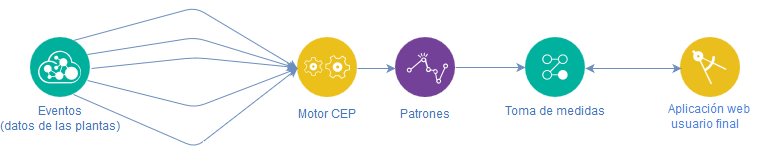
\includegraphics[width=\textwidth]{vision_general_fase_3.png}}
    \caption{esquema general para comprender mejor el objetivo que persigue el proyecto.}
    \label{fig:mesh1}
\end{figure}

En líneas generales, tendremos una serie de datos que llegarán de los campos solares, estos datos los llamaremos eventos porque son considerados sucesos que incluyen una marca de tiempo. Toda esta información se filtrará y acondicionara para el motor CEP donde estarán incluidos los patrones de eventos que desarrollaremos. Cuando el motor detecte a partir de los eventos que ha recibido un patrón se tomaran una serie de medidas, como puede ser el envío de una alerta a un técnico. Esto lo podemos ver graficamente en la figura \ref{fig:mesh1}.

\section{2. TECNOLOG\'IA ESPEC\'IFICA / INTENSIFICACIÓN / ITINERARIO CURSADO POR EL ALUMNO}
El Trabajo Fin de Grado (TFG, de ahora en adelante) siempre deber\'a demostrar la aplicaci\'on de las competencias
generales de la titulaci\'on. Adem\'as, el TFG deber\'a aplicar \textbf{algunas} de las competencias espec\'ificas
asociadas a la \textbf{Tecnolog\'ia Espec\'ifica o Intensificaci\'on} que el alumno ha cursado. Por lo tanto, el alumno
incluir\'a en el anteproyecto \textbf{dos tablas}. Una tabla para seleccionar la tecnolog\'ia cursada y en la que se
contextualiza el TFG:


\bigskip

{\centering\bfseries
Tabla 1. Tecnolog\'ia Espec\'ifica cursada por el alumno
\par}

\begin{center}
\tablefirsthead{}
\tablehead{}
\tabletail{}
\tablelasttail{}
\begin{supertabular}{m{6.803cm}}
 \rowcolor{gray!50}
{\bfseries Marcar la Tecnolog\'ia Cursada}
\\\hline
~

Tecnolog\'ias de la Informaci\'on\\
\rowcolor{gray!30}
~

Computaci\'on\\
~

Ingenier\'ia del Software \hfill x\\
\rowcolor{gray!30}
~

Ingenier\'ia de Computadores\\\hline
\end{supertabular}
\end{center}



\clearpage\pagestyle{plain}
\thispagestyle{FirstPage}

\ \ En la segunda tabla, el alumno deber\'a justificar c\'omo \textbf{algunas} de las competencias espec\'ificas de la
intensificaci\'on se aplicar\'an o tomar\'an forma en el TFG, \textbf{La relaci\'on de competencias por
intensificaci\'on se encuentran en el Anexo I al final de este documento. }


\bigskip
{\centering\bfseries
Tabla 2. Justificaci\'on de las competencias espec\'ificas abordadas en el TFG
\par}
\begin{center}
	%\newcolumntype{C}{>{\centering} m{1cm} }
  \begin{supertabular}{m{5.605cm}m{10.849cm}}
  	\iffalse
    	primera fila, cabecera
    \fi
    \rowcolor{gray!50}
	{\color{black} \textbf{Competencias}} &
	{\color{black} \textbf{Justificaci\'on}}\\\hline
    
    {\color{black} Competencia 1: capacidad para desarrollar, mantener y evaluar servicios y sistemas software que satisfagan todos los requisitos del usuario y se comporten de forma fiable y eficiente, sean asequibles de desarrollar y mantener y cumplan normas de calidad, aplicando las teor\'ias, principios, m\'etodos y pr\'acticas de la Ingenier\'ia del Software.} &
    {\color{black} La justificación de esta competencia la desmigaré en tres partes.
    {\begin{itemize} 
    \item primero la metodología de desarrollo que utilizaré será scrum junto con prototipado.
    \item Segundo, las tecnologías utilizadas serán, principalmente, el lenguaje Esper EPL y su un motor cep. Aunque esta tecnología es la piedra angular de este desarrollo, de forma secundaria necesitamos más herramientas que le provean los datos, que manejen las salidas del motor y que a todo esto le den cohesión. Por eso también utilizaremos la plataforma Anypoint de MuleSoft, la cual es un ESB (Enterprise service bus). Este ESB esta formado por flujos los cuales se pueden configurar con diferentes módulos conectables.
    \item El mantenimiento del software es algo fundamental pero debido a la naturaleza del producto que vamos desarrollar, a priori, no habrá un proceso de mantenimiento como tal. Por esta razón, tanto la documentación como el código y su configuración estarán formados teniendo siempre en mente que este código será leído y modificado por alguien diferente a mi.
    \item Para evaluar el proyecto desde el principio se aplicaran pruebas unitarias y pruebas de integración además de reuniones periodicas en las que se tendrán pruebas de aceptación por su parte.
    \end{itemize}}
    }\\
    
    \rowcolor{gray!30}
    {\color{black} Competencia 2: Capacidad para valorar las necesidades del cliente y especificar los requisitos software para satisfacer estas necesidades, reconciliando objetivos en conflicto mediante la b\'usqueda de compromisos aceptables dentro de las limitaciones derivadas del coste, del tiempo, de la existencia de sistemas ya desarrollados y de las propias organizaciones.} &
    {\color{black} Para la toma de requisitos al cliente y más adelante para que todo case se harán reuniones periódicas al principio y al final de cada iteración (y siempre que se precisen).
    La elicitación de los requisitos se hará con historias de usuario por un lado, para la parte más relacionada con la sección del sistema cercano al usuario final. Esto es así porque del resto de posibilidades que nos quedan, como pueden ser los casos de uso, no son lo más adecuado a la metodología que vamos a utilizar. Por otro lado, para recoger los patrones utilizaremos el lenguaje natural\newline
    Finalmente, para dejar claro que lo realizado en las iteraciones se ajusta a lo definido inicialmente cada historia de usuario tendrá una prueba de aceptación, relativa al prototipo que se entregue.}\\
    
    {\color{black} Competencia 3: Capacidad de dar soluci\'on a problemas de integraci\'on en funci\'on de las estrategias, est\'andares y tecnolog\'ias disponibles. } &
    {\color{black} 
    La integración del sistema dentro del entorno real será en un servidor de la empresa (propio o contratado) donde se ejecutará el software de creado. Todas las tecnologías que vayan a ser utilizadas, inicialmente, serán analizadas para comprobar que serán compatibles con el entorno final.}\\
    
    \rowcolor{gray!30}
    {\color{black} Competencia 4: Capacidad de identificar y analizar problemas y dise\~nar, desarrollar, implementar, verificar y documentar soluciones software sobre la base de un conocimiento adecuado de las teor\'ias, modelos y t\'ecnicas actuales.} &
    {\color{black}El problema que vamos a atacar es detectar ciertos desgastes y futuros fallos en todo el sistema que hay detrás de una o varias plantas fotovoltaicas. Para ello vamos a analizar todos los datos generados de las placas de estos campos. Al ser una gran cantidad, el monitóreo de las instalaciones debe de ser en tiempo real, los resultados del análisis de los datos deben de estar lo antes posible y por último inferir, a priori, inferir los datos para obtener esos resultados no es una tarea trivial, por tanto podemos decir que la opción que mejor se ajusta a estos requisitos es cep.
    
    Todo esto es relativo al tema de la tecnología que hemos visto que mejor se podría ajustar al problema que tenemos entre manos pero por muy acertado que sea cep, como sabemos, es necesario llevar a cabo un proceso de desarrollo valido y coherente. Por esto, la elicitación de requisitos (storyboards, historias de usuario y lenguaje natural), la implementación (y entregas de artefactos) y, por último, las pruebas deben de estar bien ajustadas al contexto que rodea a este proyecto.}\\
    
    {\color{black} Competencia 5: Capacidad de identificar, evaluar y gestionar los riesgos potenciales asociados que pudieran presentarse.} &
    {\color{black} A continuación, analizando las posibilidades que nos da el proyecto, el porqué se han tomado algunas decisiones de gran calado como son la implementación de cep, la metodología de desarrollo, como conectamos con los datos que se le suministraran al esb para que mas adelante el motor lo procese. El resto de tecnologías que debemos de integrar nos vienen ya impuestas por el cliente, por ejemplo la salida del flujo serán inserciones en una base de datos MySQL desde la cual una aplicacion web ya existente mostrara lo guardado (alertas/mensajes generados por el motor cep).
     seguidamente tenemos algunos de los principales moteres cep que hemos tenido en cuenta, algunos motores cep: 
      \begin{itemize}
        \item \href{https://flink.apache.org/index.html}{flint}
        \item \href{https://docs.jboss.org/drools/release/6.2.0.CR3/drools-docs/html/DroolsComplexEventProcessingChapter.html}{drools}
        \item \href{https://github.com/wso2/siddhi
    y https://wso2.com/products/complex-event-processor/}{Siddhi} and \href{https://wso2.com/products/complex-event-processor/}{WSO2}
        \item \href{https://cloud.google.com/solutions/architecture/complex-event-processing}{Google Cloud Platform}
        \item \href{http://www.oracle.com/technetwork/middleware/complex-event-processing/documentation/index.html}{Real Time Streaming Analytics Oracle}
        \item \href{http://www.espertech.com/esper/}{Esper}
      \end{itemize}
      
      Después de revisar y analizar las posibles opciones que tenemos con cep, hemos optado por Esper por las siguientes razones:
      \begin{itemize}
      \item Esper es open source, bajo la licencia GNU GPL.
      \item Esta desarrollado en Java por tanto se ajusta gratamente con el esb que comentaremos mas adelante.
      \item Este motor utiliza como lenguaje de programación de patrones Esper EPL, un lenguaje muy similar a los lenguajes SQL, con ciertas adaptaciones, como pueden ser las ventanas de tiempo, las cuales son extremadamente variadas en conparacion con otros lenguajes de la misma indole.
      \item este lenguaje es uno de los mas completos dentro de los EPLs.
      \item 
      \end{itemize}
      
      Como el sistema a desarrollar esta formado por sistemas dispares, debemos de ser capaces de hacerlos coexistir.Esto lo podemos hacer nosotros mismos o mediante el esb, con el cual conseguimos que todo este proceso se simplifique infinitamente. Por eso se ha decidido utilizar uno, ahora veremos algunas opciones que hay en el mercado actualmente de esbs:
      \begin{itemize}
      \item \href{https://www.ibm.com/support/knowledgecenter/en/SSQH9M_7.0.0/com.ibm.websphere.wesb.doc/doc/welcome_wps_ovw.html}{WebSphere Enterprise Service Bus (IBM)}
      \item \href{http://www.oracle.com/technetwork/middleware/service-bus/overview/index.html}{Oracle service bus}
      \item \href{https://developers.redhat.com/products/fuse/overview/}{Red Hat JBoss Fuse}
      \item \href{https://www.talend.com/products/application-integration/esb-open-studio/}{Talend ESB}
      \item \href{https://wso2.com/products/enterprise-service-bus/}{WSO2 ESB}
      \end{itemize}
      En el siguiente listado vemos las ventajas de Mule, porque hemos optado por él y no por otros esbs:
      \begin{itemize}
      \item A parte de la gran cantidad de componentes que tiene, mediante el componente de Java se le pueden integrar y adaptar infinidad de sistemas, librerias, framworks y todo lo que se nos ocurra. Podríamos decir que se le puede conectar casi todo.
      \item el paso de mensajes entre componentes puede ser en cualquier formato, no fuerza a utilizar Json o xml, entre otros.
      \item Su arquitectura lo hace muy escalable.
      \item El proyecto es open source.
      \item Tiene dos versiones, la enterprise, de pago y la community, gratuita.
      \item Una gran documentación con muchos tutoriales y un foro con una importante comunidad detrás.
      \end{itemize}
   	}\\
    
    \rowcolor{gray!30}
    {\color{black} Competencia 6: Capacidad para dise\~nar soluciones apropiadas en uno o m\'as dominios de aplicaci\'on utilizando m\'etodos de la ingenier\'ia del software que integren aspectos \'eticos, sociales, legales y econ\'omicos.} &
    {\color{black} Para poder llevar a buen puerto este proyecto y que alcance los objetivos que nos hemos planteado es preciso diseñar una una hoja de ruta,una planificación, que nos asegure este propósito. Para ello teniendo en cuenta todos los condicionantes que nos rodean, la opción que creemos mas viable es definir en tres grandes iteraciones o fases el proyecto. Cada una de ella estará a su vez dividida en varios springs mas cortos, de una semana. La primera fase, relacionada con la toma y elicitación de requisitos y diseño. La segunda ya incluye implementación, testeo y entrega de un primer prototipo capaz de detectar patrones y notificarlos a a partir de datos ya recolectados y almacenados. La tercera fase incluirá una revisión de patrones, pudiendo añadir alguno nuevo; y se desarrollará el adaptador para que los datos finalmente provengan en tiempo real, saliendo de esta última iteración la entrega definitiva.
    }\\

\end{supertabular}
\end{center}
\bigskip

\section{3. \ OBJETIVOS}
Siendo concisos, el objetivo principal de este trabajo es conseguir analizar una serie de datos, obtenidos de una serie de plantas fotovoltaicas, en tiempo real para obtener una serie de alertas, recomendaciones o acciones. De esta forma subsanar fallos o averías, pero no solo en el presente sino también predecirlas en el futuro.

Esto se puede dividir en 4 sub-objetivos, los cuales son:

\begin{itemize}
	\item Creación de un adaptador al flujo de datos que nos proporcione Ingeteam. \newline
    \textbf{Limitaciones y condicionantes:} en este sub-objetivo tenemos una limitación importante y es que por parte de ingeteam, no todas las plantas nos pueden proporcionar los datos en tiempo real ya que algunas de ellas no son ellos los propietarios.\newline 
    \textbf{Sobre la tecnología:} esta mas que probada y lleva ya bastantes años en funcionamiento con una gran documentación y comunidad detrás.
    
    \item Obtención, diseño e implementación de patrones complejos.
    \textbf{Limitaciones y condicionantes:} los datos que emanan de las plantas en algunos casos no es trivial su análisis, es decir, detectar que datos, de forma conjunta e interrelacionado de una manera especifica, podrían ser un patrón interesante. La solución a esto pasa casi por la prueba y error. (Una de las razones por las que se ha decidido utilizar scrum y prototipado).
    \textbf{Sobre la tecnología:} para el diseño no será necesaria ninguna tecnología especifica pero para su implementación si que deberemos de hacer uso del ya mencionado Esper EPL, siendo este una de las mejores opciones como ya hemos comentado en el listado de sus ventajas.
    
    \item Crear las respuestas a los patrones detectados.
    \textbf{Limitaciones y condicionantes:} aunque es un objetivo que debemos de alcanzar el como no esta definido completamente, en otras palabras, Ingeteam debe de definirnos que quieres que hagamos con los patrones detectados. Inicialmente nos comentaron de insertar en su base de datos de alertas. Hasta donde sabemos la base de datos es MySQL, cuya configuración por nuestra parte no debe de ser complicada gracias a enorme cantidad de tutoriales y documentación.
    
    \item Integración de todos los sistemas necesarios.
    \textbf{Limitaciones y condicionantes:} en un principio esta es la parte que mas atada esta, las pruebas que se han hecho con el esb parecen bastante satisfactorias. Evidentemente, aunque aun no hemos tenido problemas, es el paso mas crítico ya que debe de aunar una gran cantidad de lenguajes, librerias, el motor cep y conexiones a sistemas externos.
    \textbf{Sobre la tecnología:} para llevar a cabo esto utilizaremos Anypoint Studio junto con mule, con los que no hemos tenido problema alguno creando flujos de datos.

\end{itemize}
De acuerdo a la Introducci\'on, el alumno deber\'a especificar cu\'al o cuáles son las hip\'otesis de trabajo de las
que se parten, qu\'e se pretende resolver, y en base a eso formular el objetivo principal del TFG.

El objetivo principal deber\'a desglosarse en sub-objetivos parciales. Los sub-objetivos deberán describirse de forma breve y concisa.

Como pre\'ambulo a la formulaci\'on del objetivo parcial, el alumno deber\'a discutir sobre las limitaciones y
condicionantes a tener en cuenta en el desarrollo del TFG (lenguaje de desarrollo, equipos, madurez de la tecnolog\'ia,
etc.).

Del mismo modo, ser\'a recomendable incluir una lista preliminar de requisitos del sistema a construir.

\section[4. M\'ETODO Y FASES DE TRABAJO]{4. M\'ETODO Y FASES DE TRABAJO}

\bigskip

\subsection{Justificación de la metodología}
Como adelantamos en las competencias la metodología por la que hemos optado es scrum junto con prototipado. La elección de esta no es por capricho sino por necesidad, y esta completamente justificado su uso como ahora veremos. El proceso de elección comenzó preguntándonos por el tipo de metodología, a saber, las tradicionales o ágiles. La principal razón por la que se decidió tomar una metodología ágil es simple, tendremos una gran cantidad de cambios (sobre todo en los patrones) e, incluso, cierta incertidumbre. Como es sabido esta este es el talón de aquiles de las metodología mas convencionales. Aunque es una importante razón también optamos por una metodología ágil porque la productividad se ve aumentada, la producción ira mas rápida, la calidad del producto es mayor y todo esto se traduce en una mayor satisfacción en los stakeholders (poner la referencia al libro de la biblioteca) Decidido esto teníamos que escoger una de las muchas y variadas metodologías ágiles por las que podemos optar. Finalmente nos decantamos por scrum por varias razones, tiene una gran documentación sobre su aplicabilidad, hay gran cantidad de herramientas diseñadas para utilizarla, en comparación con otras metodologías ágiles, scrum es de las que mejor se adaptan al cambio, en proyectos con tecnologías nuevas donde existe una curva de aprendizaje por parte de los componentes del equipo de desarrollo y por último, el producto debe de ser lanzado en partes desde que se comienza el desarrollo.

\subsection{Planificación estimada}

Como ya he comentado el proyecto estará divido en tres fases principales. La primera incluye una serie de tareas de elicitación y diseño, por otro lado también se iniciará el desarrollo de este documento. A partir de las reuniones con los responsables de Ingeteam se diseñara la arquitectura de todo el sistema, desde como se cogen los datos hasta que se da una salida. Lo siguiente es crear una demo sobre como funcionará el programa final. Cuando todo esto haya quedado fijado instalaremos todas las herramientas, librerías y componentes necesarios, estos son el repositorio para guardar el código generado, el entorno en VSTS (Visual Studio Team Services) para controlar el tablero de scrum y todo lo relacionado con la documentación, instalaremos también Medit4CEP, herramienta que agiliza el diseño de los patrones, La librería POI para leer de ficheros excel, el motor Esper, el entorno para Mule Anypoint Studio, la librería para conectarnos a bases de datos MySQL.

La segunda fase estará dominada por el desarrollo del producto. A partir de la demo creada en la fase anterior se le añadiran nuevas modificaciones, que lea de los ficheros excel los datos necesarios. El uso del motor Esper con patrones más complejos e interesantes propuestos hasta la fecha. El diseño de los patrones con Medit4CEP. Inserción de los resultados de los patrones en la base de datos indicada por Ingeteam en la forma que nos especifiquen.

En la tercera fase estaremos mas centrados en el mantenimiento de lo desarrollado, modificando los patrones ya creados y añadiendo nuevos. (se hara una pequeña interfaz para añadir nuevos patrones/tipos de datos de entrada?)

Durante todo este proceso de creación se realizaran tareas de testeo de todos los productos generados

Como parte de la descripci\'on del m\'etodo y las fases de trabajo, el alumno podr\'a incluir una descripci\'on
preliminar de las tareas, una planificaci\'on temporal, diagramas de Gantt o recursos similares que pueda considerar
necesarios.

Si hubiera m\'as de una metodolog\'ia que a juicio del alumno podr\'ia ser af\'in al proyecto, \'estas deber\'an
mencionarse, y justificar la que considera m\'as adecuada (esto puede considerarse parte de la justificaci\'on a la
adecuaci\'on al problema a resolver).

\section{5. MEDIOS QUE SE PRETENDEN UTILIZAR}
\section{5.1. Medios Hardware}

El proyecto es meramente software por tanto no sera necesario ningún tipo de hardware, más allá de la maquina que ejecutará el sistema. (poner los requisitos mínimos y donde funcionaría bien?)

\section{5.2. Medios Software}

El alumno deber\'a describir los medios software (lenguajes, entornos de desarrollo, herramientas de gesti\'on y
planificaci\'on, etc.) que prev\'e ser\'an necesarios para el desarrollo del proyecto

\textbf{lenguajes}
\begin{itemize}
\item Esper EPL: es el lenguaje con el que se crearan los patrones de eventos que serán detectados
\item Java: todas las funcionalidades que no estén ya implementadas estarán codificadas en este lenguaje como puede ser el lector de ficheros excels.
\item SQL: el subconjunto que implementa el gestor de bases de datos MySQL. Será utilizado para acceder a la bases de datos que tendremos en la parte final de nuestro flujo.
\end{itemize}

\textbf{Librerías}
\begin{itemize}
\item Esper EPL engine: se encargará de poder ejecutar los patrones teniendo en cuenta los datos que le entren.
\item MySQL connection java: para poder conectar desde Mule a un servidor MySQL.
\item POI: libreria para java muy útil para poder leer los datos de los ficheros excel.
\end{itemize}

\textbf{Entornos}
\begin{itemize}
\item Mule: fundamental para poder dar cohesión a toda esta gran cantidad de elementos software de una forma sencilla e incluso visual.
\item Medit4CEP: indispensable para diseñar visualmente y generar los patrones de eventos que utilizaremos mas adelante.
\item GitHub Desktop: gestor de repositorios gráfico de la página homónima, con realizaré el mantenimiento de todo el código del proyecto.
\end{itemize}

\textbf{Herramientas de gestión y planificación}
\begin{itemize}
\item VSTS(Visual Studio Team Servicies): con ella llevaremos a cabo todo lo relacionado con la genstion de las iteraciones y tableros de la metodología scrum.
\item repositorio en GitHub: en el guardare todo el código generado en el proyecto.
\end{itemize}

%\clearpage\pagestyle{empty}
%\thispagestyle{FirstPage}

\section[6. REFERENCIAS]{6. REFERENCIAS}
En esta secci\'on se incluir\'an todas las referencias bibliogr\'aficas, ordenadas alfab\'eticamente por el primer
apellido del primer autor, de las obras de las cuales se haya realizado alguna cita en los apartados anteriores. Las
referencias deber\'an contener datos b\'asicos como nombre y apellidos de los autores, t\'itulo de la obra, evento al
que pertenece, p\'aginas, fecha y lugar de celebraci\'on (si se tratara de art\'iculos de congreso), ISBN, editorial y
ciudad (si se tratara de libro), nombre de revista, p\'aginas, volumen y n\'umero (si se tratara de revista), etc.

Se emplear\'a un formato de referencia reconocido en el \'ambito acad\'emico como
ACM\footnote{http://www.acm.org/sigs/publications/proceedings-templates}\footnote{http://www.cs.ucy.ac.cy/\~{}chryssis/specs/ACM-refguide.pdf}.
Otros formatos aconsejables son, por ejemplo, IEEE, AMA, APA y AMA.

Ejemplos de referencias con formato ACM:

\liststyleLi
\begin{itemize}
\item Para un art\'iculo de revista:
\end{itemize}
Bowman, M., Debray, S. K., and Peterson, L. L. 1993. Reasoning about naming systems. \textit{ACM Trans. Program. Lang.
Syst.} 15, 5 (Nov. 1993), 795-825. DOI= \url{http://doi.acm.org/10.1145/161468.16147}.

\liststyleLii
\begin{itemize}
\item Para un informe t\'ecnico
\end{itemize}
Ding, W. and Marchionini, G. 1997. \textit{A Study on Video Browsing Strategies. Technical Report}. University of
Maryland at College Park.

\liststyleLiii
\begin{itemize}
\item Para un libro

Tavel, P. 2007. \textit{Modeling and Simulation Design.} AK Peters Ltd., Natick, MA, USA.
\end{itemize}
\liststyleLiv
\begin{itemize}
\item Para un cap\'itulo de libro:
\end{itemize}
Greiner, R. 1999. Explanation-based learning. In Wilson and F. Keil, R. eds. \textit{The Encyclopedia of Cognitive
Science}, MIT Press, Cambridge, MA, USA. 301-303.

\liststyleLv
\begin{itemize}
\item Para un art\'iculo en las actas de un congreso:
\end{itemize}
Fr\"ohlich, B. and Plate, J. 2000. The cubic mouse: a new device for three-dimensional input. In \textit{Proceedings of
the SIGCHI Conference on Human Factors in Computing Systems} (The Hague, The Netherlands, April 01 - 06, 2000). CHI
'00. ACM, New York, NY, 526-531. DOI= \url{http://doi.acm.org/10.1145/332040.332491}.

\liststyleLvi
\begin{itemize}
\item Para un p\'agina de Internet (con autores conocidos)

Steele, B. Look, Ma, no wires! Cornell class project tests wireless networking, \textit{Cornell Chronicle, 31 }(35).
Retrieved February 15, 2004, from Columbia University:
\url{http://www.news.cornell.edu/Chronicle/00/5.18.00/wireless_class.html}
\item Para un p\'agina de Internet (con autores desconocidos)

MIT Project Oxygen: Overview, 2004. Retrieved March 15, 2005, from Computer Science and Artificial Intelligence
Laboratory, Massachusetts Institute of Technology: \url{http://oxygen.lcs.mit.edu/Overview.html}. \
\end{itemize}

\bigskip

\clearpage\clearpage\pagestyle{plain}
\thispagestyle{FirstPage}


\bigskip
\end{document}
